% Composing metasurfaces from measured meta-atoms — method, results, the
% a,b;c,d / atom-D failures, the algorithmic limit, and why the fix is not
% in the aggregation.
%
% Compile with pdflatex (twice).  Figures are the cropped panels in figs/;
% compile from this directory:  pdflatex tmatrix_composed_metasurfaces.tex
\documentclass[10pt,aspectratio=169]{beamer}

\usepackage[T1]{fontenc}
\usepackage[utf8]{inputenc}
\usepackage{lmodern}
\usepackage{amsmath,amssymb}
\usepackage{booktabs}
\usepackage{graphicx}
\usepackage{xcolor}
\usepackage{tikz}
\usepackage{textcomp}

% ---------------------------------------------------------------- palette
\definecolor{navy}{RGB}{21,34,56}
\definecolor{ink}{RGB}{31,41,55}
\definecolor{gold}{RGB}{183,121,31}
\definecolor{golddk}{RGB}{140,90,19}
\definecolor{good}{RGB}{46,125,50}
\definecolor{warn}{RGB}{180,83,9}
\definecolor{bad}{RGB}{192,57,43}
\definecolor{cardbg}{RGB}{244,246,248}
\definecolor{cardgold}{RGB}{250,243,227}

\usetheme{default}
\usecolortheme{seagull}
\setbeamercolor{structure}{fg=navy}
\setbeamercolor{frametitle}{fg=navy,bg=white}
\setbeamercolor{title}{fg=white}
\setbeamercolor{subtitle}{fg=gold}
\setbeamercolor{normal text}{fg=ink}
\setbeamerfont{frametitle}{series=\bfseries,size=\large}
\setbeamertemplate{navigation symbols}{}
\setbeamertemplate{itemize item}{\textcolor{gold}{\raisebox{0.12ex}{\scriptsize$\bullet$}}}
\setbeamertemplate{itemize subitem}{\textcolor{golddk}{--}}
\setbeamertemplate{footline}{%
  \hfill{\scriptsize\textcolor{gray}{Composing metasurfaces from measured meta-atoms\quad
  \textcolor{gold}{\bfseries\insertframenumber\,/\,\inserttotalframenumber}}}\hspace{2mm}\vspace{1mm}}

\newcommand{\kicker}[1]{{\footnotesize\bfseries\textcolor{gold}{#1}}\\[-0.4ex]}
\newcommand{\um}{\,\text{\textmu m}}

\title{Composing Metasurfaces from Measured Meta-Atoms}
\subtitle{T-matrix pipeline: method, validation, and a diagnosed limit}
\author{DaryLu0v0}
\institute{\texttt{D:\textbackslash Claude\textbackslash T matrix}  $\cdot$  ten direct-CST benchmarks  $\cdot$  cross-verified against treams (KIT) to $10^{-12}$}
\date{August 2026}

\begin{document}

% ================================================================ 1 title
{\setbeamercolor{background canvas}{bg=navy}
\begin{frame}[plain]
  \vspace{1.2cm}
  {\footnotesize\bfseries\textcolor{gold}{T-MATRIX PIPELINE  $\cdot$  METHOD, VALIDATION, AND A DIAGNOSED LIMIT}}\\[2ex]
  {\LARGE\bfseries\textcolor{white}{Composing Metasurfaces from\\Measured Meta-Atoms}}\\[3ex]
  {\normalsize\textcolor{white!80!navy}{Extract each meta-atom's transition matrix from one full-wave simulation, then predict whole
  metasurfaces by linear algebra --- where that works, where it breaks, and why the break is not
  fixable inside the aggregation algorithm.}}\\[3ex]
  {\color{gold}\rule{4cm}{1pt}}\\[1ex]
  {\small\textcolor{white!60!navy}{\texttt{D:\textbackslash Claude\textbackslash T matrix}  $\cdot$ 
  ten direct-CST benchmarks  $\cdot$  cross-verified against treams (KIT) to $10^{-12}$  $\cdot$  August 2026}}
\end{frame}}

% ================================================================ 2 the idea
\begin{frame}{One full-wave solve per atom --- then metasurfaces become linear algebra}
  \kicker{METHOD  $\cdot$  1 OF 2}
  \begin{columns}[t]
    \begin{column}{0.32\textwidth}
      \textcolor{navy}{\textbf{1\quad Extract}}\hfill{\scriptsize\textit{\textcolor{golddk}{once per meta-atom}}}
      \begin{itemize}\footnotesize
        \item One CST solve of the isolated atom (PML, plane-wave illumination set)
        \item Near fields sampled on a sphere, projected onto vector spherical waves (VSWFs)
        \item Least-squares fit $F = T\,A$ $\rightarrow$ the atom's transition matrix $T$ ($30\times 30$ at $l_{\max}=3$)
      \end{itemize}
    \end{column}
    \begin{column}{0.32\textwidth}
      \textcolor{navy}{\textbf{2\quad Aggregate}}\hfill{\scriptsize\textit{\textcolor{golddk}{per arrangement}}}
      \begin{itemize}\footnotesize
        \item Place measured atoms on any periodic cell --- one species or several
        \item Pair-resolved Ewald lattice sums couple every atom to every other, exactly
        \item Solve the block Foldy--Lax system for the self-consistent excitations
      \end{itemize}
    \end{column}
    \begin{column}{0.32\textwidth}
      \textcolor{navy}{\textbf{3\quad Predict}}\hfill{\scriptsize\textit{\textcolor{golddk}{milliseconds each}}}
      \begin{itemize}\footnotesize
        \item Project onto Floquet orders $\rightarrow$ full complex S-parameters, all diffraction channels
        \item No full-wave simulation of the composed array is ever run
        \item 64\,min of CST per supercell benchmark vs milliseconds per composed design
      \end{itemize}
    \end{column}
  \end{columns}
  \vspace{2ex}
  \begin{beamercolorbox}[rounded=true,sep=6pt]{block body}
    \colorbox{cardgold}{\parbox{0.96\textwidth}{\small\textbf{\textcolor{golddk}{The promise:}}
    simulate each atom once, then compose arbitrarily many metasurfaces from the measured parts ---
    the repeated cell may hold one meta-atom or several different ones.}}
  \end{beamercolorbox}
\end{frame}

% ================================================================ 3 the algebra
\begin{frame}{The algebra: block-Bloch Foldy--Lax with Ewald lattice sums}
  \kicker{METHOD  $\cdot$  2 OF 2}
  \begin{columns}[t]
    \begin{column}{0.52\textwidth}
      {\scriptsize\textcolor{golddk}{\textbf{Atom response (VSWF basis)}}}
      \begin{equation*} p = T\,a \end{equation*}
      {\scriptsize\textcolor{golddk}{\textbf{Pair-resolved Bloch lattice sum (Ewald)}}}
      \begin{equation*}
        W_{st}(\mathbf{k}_\parallel) \;=\; {\sum_{\mathbf{R}}}'\;
        A(\boldsymbol{\rho}_t - \boldsymbol{\rho}_s + \mathbf{R})\,
        e^{\,i \mathbf{k}_\parallel \cdot \mathbf{R}}
      \end{equation*}
      {\scriptsize\textcolor{golddk}{\textbf{Self-consistent block solve, $M$ atoms per cell}}}
      \begin{equation*}
        (I - W\,T)\,a = a_{\text{inc}}, \qquad f = T\,a
      \end{equation*}
      {\scriptsize\textcolor{golddk}{\textbf{Floquet output map, order $\mathbf{G}$ on either side}}}
      \begin{equation*}
        E_{\mathbf{G}} \;\propto\; \frac{1}{k_{z,\mathbf{G}}} \sum_s
        e^{-i \mathbf{k}_{\mathbf{G}} \cdot \boldsymbol{\rho}_s}\,
        F_s(\hat{\mathbf{k}}_{\mathbf{G}})
      \end{equation*}
    \end{column}
    \begin{column}{0.44\textwidth}
      \begin{itemize}\small
        \item Basis: vector spherical waves to $l_{\max}=3$ $\rightarrow$ 30 modes per atom; a four-atom cell is a dense $120\times120$ solve.
        \item Lattice sums by Ewald summation (via treams); an $\eta$-stability bracket refuses rather than guesses when the split disagrees.
        \item Conventions measured identical to treams: VSWFs to $7\times10^{-16}$, plane-wave expansion $6\times10^{-16}$, translation operator $5\times10^{-15}$.
        \item Every propagating diffraction order is returned, power-normalized --- supercells diffract inside the band.
      \end{itemize}
    \end{column}
  \end{columns}
\end{frame}

% ================================================================ 4 the experiment
\begin{frame}{Four measured gold meta-atoms, ten blind CST benchmarks}
  \kicker{THE EXPERIMENT}
  \begin{columns}[t]
    \begin{column}{0.48\textwidth}
      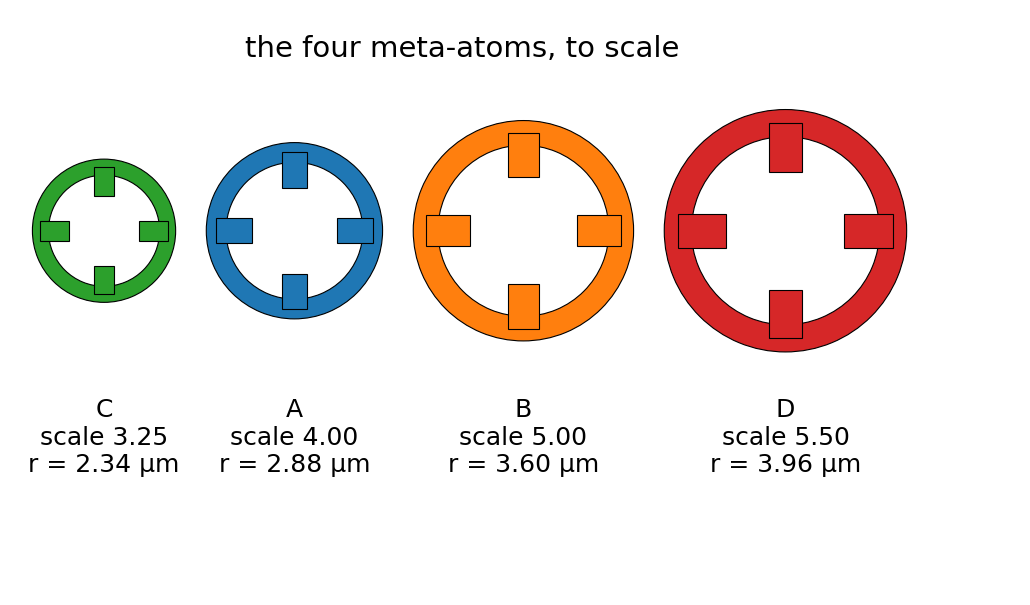
\includegraphics[width=\textwidth]{figs/atoms_to_scale.png}
      {\scriptsize\textit{\textcolor{gray}{The four spoke-and-wheel resonators, drawn to scale. All are 0.2\um-thick gold,
      extracted in isolation over 10--34\,THz (25 frequencies, stored at $l_{\max}=5$).}}}
    \end{column}
    \begin{column}{0.48\textwidth}
      \begin{center}\small
      \begin{tabular}{@{}lccc@{}}
        \toprule
        atom & scale & ring outer radius & isolated resonance / scale \\
        \midrule
        C & 3.25 & 2.338\um & 3.766 \\
        A & 4.00 & 2.877\um & 3.770 \\
        B & 5.00 & 3.596\um & 3.786 \\
        D & 5.50 & 3.956\um & 3.782 \\
        \bottomrule
      \end{tabular}
      \end{center}
      \begin{itemize}\footnotesize
        \item Layout: $16\times16\um$ repeated cell, atoms on the 8\um{} square sub-lattice --- four single-atom lattices $+$ six mixed supercells.
        \item Every case has an independent direct-CST periodic reference: ten blind benchmarks in all.
        \item Input imperfections are measured, not assumed: the extracted $T$'s violate passivity by 2--5\,\% and reciprocity by up to ${\sim}18\,\%$ --- the inputs, not the aggregation, set the error floor of the good cases.
      \end{itemize}
    \end{column}
  \end{columns}
\end{frame}

% ================================================================ 5 aggregation exact
\begin{frame}{The aggregation itself is exact to round-off}
  \kicker{VALIDATION  $\cdot$  THE CODE}
  \begin{columns}[t]
    \begin{column}{0.60\textwidth}
      \small
      \begin{tabular}{@{}lr@{}}
        \toprule
        algebraic identity / independent implementation & residual \\
        \midrule
        $M=1$ cell reduces to the one-atom code & \textcolor{good}{\textbf{bit-identical}} \\
        $2\times2$ cell of four identical atoms $\equiv$ primitive lattice & \textcolor{good}{$\le 8\times10^{-16}$} \\
        basis-atom relabelling / whole-cell lattice shift & \textcolor{good}{$\le 7\times10^{-16}$ / $0$} \\
        selection rule: power in odd $(n_1{+}n_2)$ orders & \textcolor{good}{$\le 6\times10^{-33}$} \\
        all $T=0$ $\rightarrow$ $S = S_{\text{background}}$ exactly & \textcolor{good}{$0$} \\
        independent treams chain, every cell, complex $S$ & \textcolor{good}{$\le 1\times10^{-12}$} \\
        \bottomrule
      \end{tabular}
    \end{column}
    \begin{column}{0.36\textwidth}
      \textcolor{navy}{\textbf{What this rules out}}
      \begin{itemize}\small
        \item coding errors in the block solve
        \item lattice-sum convergence
        \item basis conventions and normalization
        \item the Floquet output map
      \end{itemize}
    \end{column}
  \end{columns}
  \vspace{2ex}
  \colorbox{cardgold}{\parbox{0.96\textwidth}{\small\textbf{\textcolor{golddk}{Consequence:}}
  whatever error remains against full-wave CST lives in what a truncated single-centre T-matrix can
  \emph{represent} --- not in the code that manipulates it.}}
\end{frame}

% ================================================================ 6 results table
\begin{frame}{Accuracy is ordered by one geometric number, $\rho = (a_i + a_j)/d$}
  \kicker{RESULTS  $\cdot$  TEN BENCHMARKS}
  \begin{columns}[t]
    \begin{column}{0.50\textwidth}
      \footnotesize
      \begin{tabular}{@{}lcccl@{}}
        \toprule
        case & $\rho$ & MSE $S_{21}$ & mean $|\Delta S_{21}|$ & verdict \\
        \midrule
        C alone   & 0.584 & 0.00038 & 0.017 & \textcolor{good}{good} \\
        a,c;c,a   & 0.652 & 0.00067 & 0.019 & \textcolor{good}{good} \\
        A alone   & 0.719 & 0.00107 & 0.030 & \textcolor{good}{good} \\
        b,c;c,b   & 0.742 & 0.00171 & 0.036 & \textcolor{good}{good} \\
        a,b;b,a   & 0.809 & 0.00367 & 0.046 & \textcolor{good}{good} \\
        a,d;b,c   & 0.854 & 0.0118  & 0.080 & \textcolor{warn}{degrading} \\
        B alone   & 0.899 & 0.0039  & 0.054 & \textcolor{warn}{degrading} \\
        a,c;d,b   & 0.944 & 0.1207  & 0.244 & \textcolor{bad}{\textbf{broken}} \\
        a,b;c,d   & 0.944 & 0.1654  & 0.308 & \textcolor{bad}{\textbf{broken}} \\
        D alone   & 0.989 & 0.0351  & 0.149 & \textcolor{bad}{\textbf{broken}} \\
        \bottomrule
      \end{tabular}\\[1ex]
      {\scriptsize\textit{\textcolor{gray}{MSE $=$ mean $|S_{21}^{\text{pred}} - S_{21}^{\text{CST}}|^2$ over the band, complex amplitude, 0th order.
      Seven of ten land at mean $|\Delta S_{21}|$ 0.017--0.080 --- the level set by the input T-matrices.}}}
    \end{column}
    \begin{column}{0.46\textwidth}
      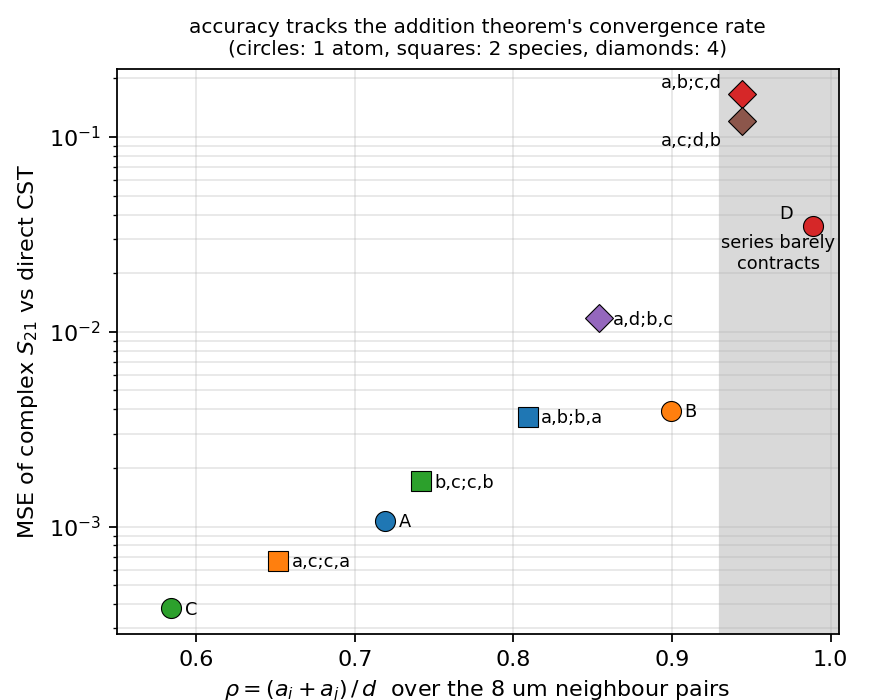
\includegraphics[width=\textwidth]{figs/mse_vs_rho.png}
      {\scriptsize\textit{\textcolor{gray}{Same data: MSE vs $\rho$. Above $\rho \approx 0.94$ (shaded) the multipole series barely contracts.}}}
    \end{column}
  \end{columns}
\end{frame}

% ================================================================ 7 what works
\begin{frame}{Where $\rho$ is moderate, composition is essentially free}
  \kicker{RESULTS  $\cdot$  WHAT WORKS}
  \begin{columns}[t]
    \begin{column}{0.50\textwidth}
      \begin{itemize}\small
        \item Seven of ten benchmarks: mean $|\Delta S_{21}|$ 0.017--0.080 --- within the input T-matrices' own passivity / reciprocity error.
        \item The supercell step adds nothing: a,b;b,a lands at 0.046, between its two pure lattices (0.030 and 0.054).
        \item A \textbf{dark lattice resonance at 16.00\um} --- invisible to any single-atom model --- was predicted and then confirmed by direct CST: dark-channel power $1.5\times10^{-5}$ against a 0.987 carrier.
        \item Its transmission window: predicted 15.57\um{} / $|S_{21}|$ 0.68, measured 15.35\um{} / 0.72.
        \item Exact selection rule (odd diffraction orders extinguished) confirmed in every cell.
      \end{itemize}
    \end{column}
    \begin{column}{0.46\textwidth}
      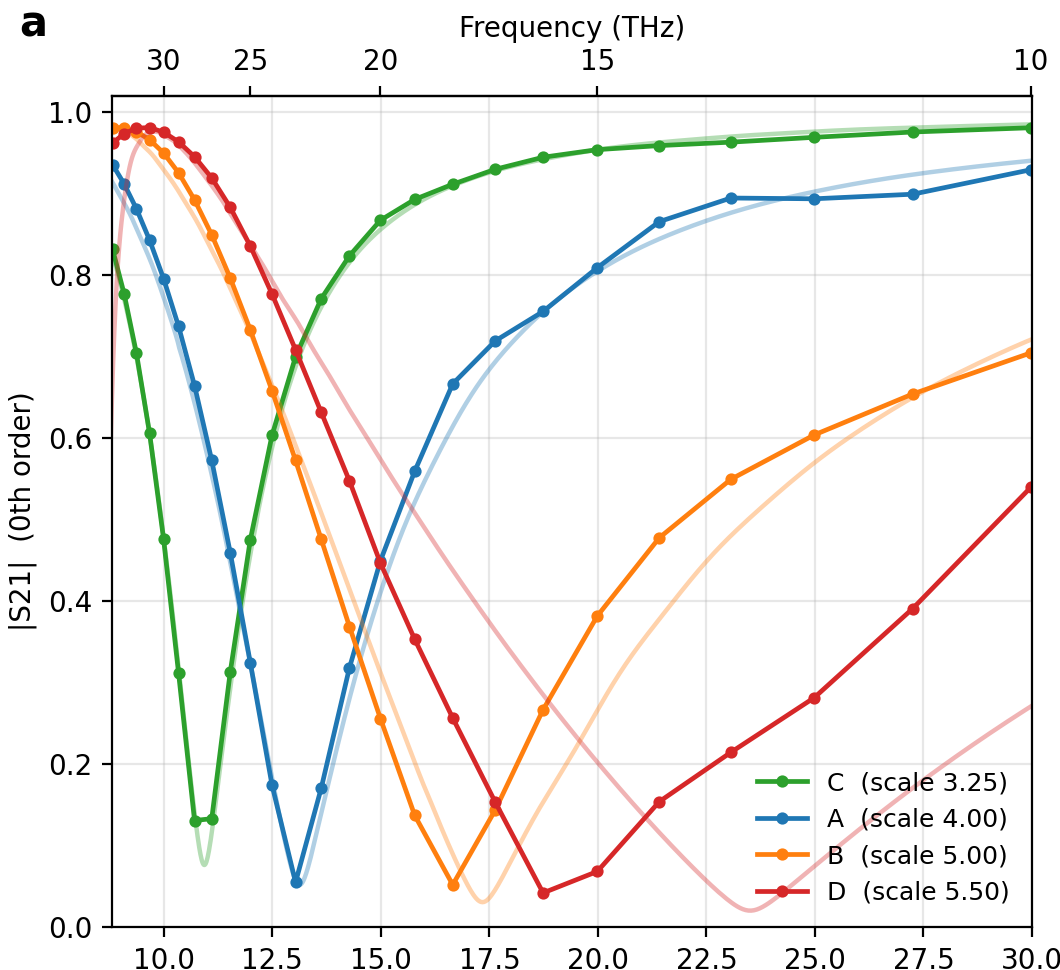
\includegraphics[width=\textwidth]{figs/s21_singles.png}
      {\scriptsize\textit{\textcolor{gray}{One atom per 8\um{} cell: prediction (markers) vs direct CST (pale).
      C, A, B track closely --- D, the largest, already fails.}}}
    \end{column}
  \end{columns}
\end{frame}

% ================================================================ 8 failure 1
\begin{frame}{Failure 1 --- same atoms, same lattice, $14\times$ worse when B and D become neighbours}
  \kicker{FAILURE 1  $\cdot$  THE A,B;C,D SUPERCELL}
  \begin{columns}[t]
    \begin{column}{0.46\textwidth}
      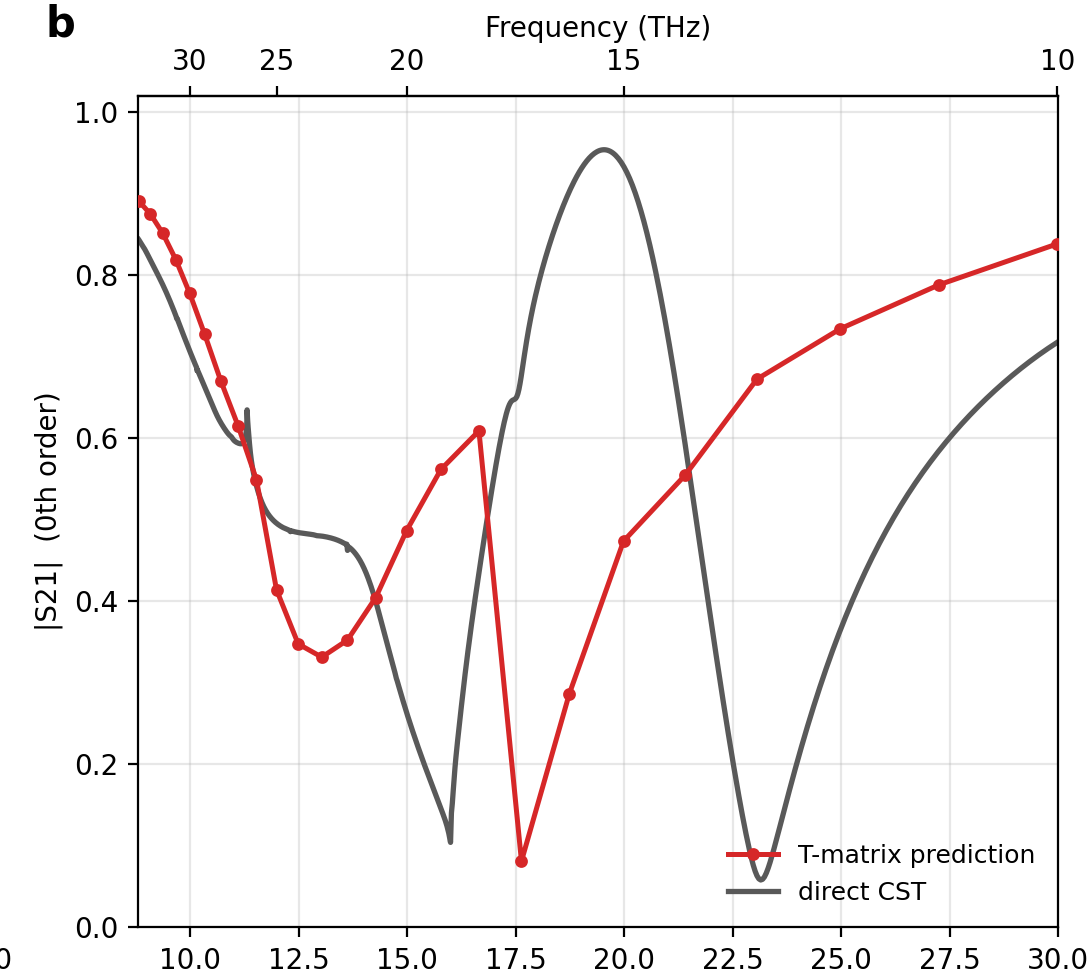
\includegraphics[width=\textwidth]{figs/s21_abcd_vs_cst.png}
      {\scriptsize\textit{\textcolor{gray}{a,b;c,d: predicted $|S_{21}|$ (red) vs direct CST (grey).
      The deepest dip is misplaced by $-5.51\um$.}}}
    \end{column}
    \begin{column}{0.50\textwidth}
      {\large\textcolor{bad}{\textbf{MSE 0.1654}}}\\
      {\small vs 0.0118 for a,d;b,c --- identical atoms, identical lattice, different adjacency}\\[2ex]
      {\large\textcolor{bad}{\textbf{$-5.51\um$ / $+4.92\um$}}}\\
      {\small dip misplacement in a,b;c,d and its $\rho$-twin a,c;d,b --- opposite signs, so no calibratable bias}\\[2ex]
      {\large\textcolor{good}{\textbf{0.409 vs 0.388}}}\\
      {\small total diffracted power of a,b;c,d, predicted vs measured (5.4\,\%); the $\rho$-twin a,c;d,b keeps 1.0\,\% (0.407 vs 0.403) --- the specular channel breaks first}
    \end{column}
  \end{columns}
\end{frame}

% ================================================================ 9 failure 2
\begin{frame}{Failure 2 --- atom D alone: the resonance lands 19\,\% away, and red-shifted}
  \kicker{FAILURE 2  $\cdot$  ATOM D'S OWN LATTICE}
  \begin{columns}[t]
    \begin{column}{0.48\textwidth}
      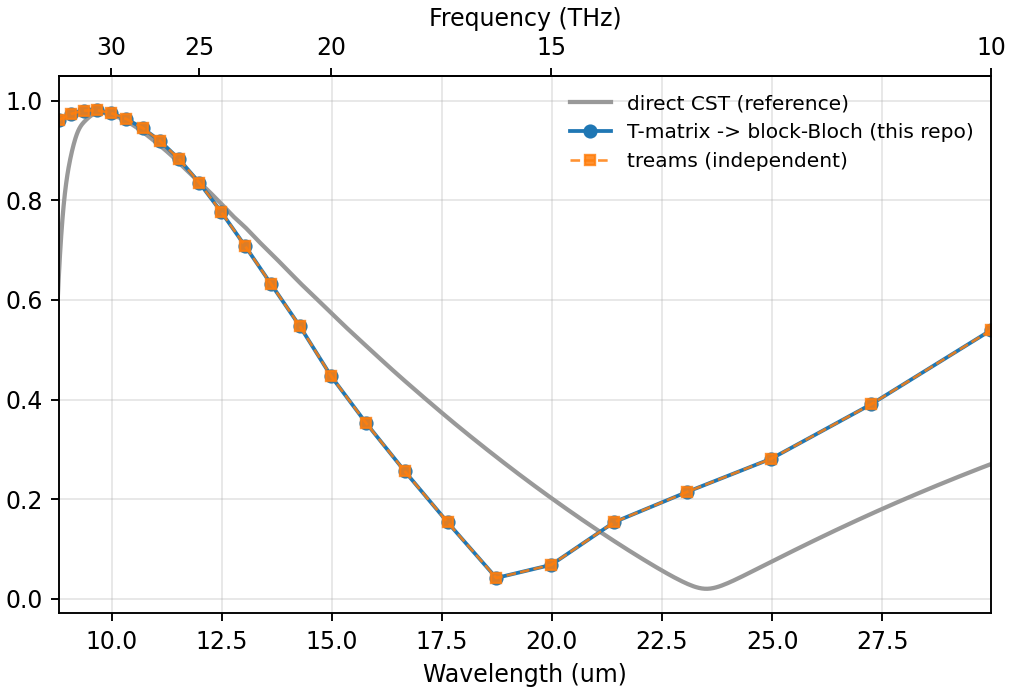
\includegraphics[width=\textwidth]{figs/s21_D_alone.png}
      {\scriptsize\textit{\textcolor{gray}{D alone on its 8\um{} lattice: predicted dip 19.1\um{} (repo $=$ treams,
      indistinguishable) vs 23.5\um{} measured; absorption goes negative.}}}
    \end{column}
    \begin{column}{0.48\textwidth}
      {\small A, B, C blue-shift from isolated to array resonance by a consistent 1.3--2.0\um.
      D red-shifts by $+2.74\um$ --- opposite sign. The anomaly tracks the closing gap, not the atom:}\\[1ex]
      \begin{center}\footnotesize
      \begin{tabular}{@{}cccc@{}}
        \toprule
        scale & gap to neighbour & CST array dip & dip / scale \\
        \midrule
        4.00 & 2.246\um & 13.13\um & 3.283 \\
        4.50 & 1.526\um & 14.90\um & 3.311 \\
        5.00 & 0.807\um & 17.34\um & 3.468 \\
        \textcolor{bad}{\textbf{5.50 (=D)}} & \textcolor{bad}{\textbf{0.088\um}} & \textcolor{bad}{\textbf{23.51\um}} & \textcolor{bad}{\textbf{4.275}} \\
        \bottomrule
      \end{tabular}
      \end{center}
      \vspace{1ex}
      \colorbox{cardgold}{\parbox{0.95\textwidth}{\footnotesize\textbf{\textcolor{golddk}{88\,nm apart at scale 5.5:}}
      the classic near-touching capacitive red-shift --- a hybridized gap mode of the pair.
      Real physics, present in full-wave, absent from the prediction.}}
    \end{column}
  \end{columns}
\end{frame}

% ================================================================ 10 suspects cleared
\begin{frame}{The T-matrix is innocent --- and so is the implementation}
  \kicker{DIAGNOSIS  $\cdot$  CLEARING SUSPECTS}
  \begin{columns}[t]
    \begin{column}{0.46\textwidth}
      \textcolor{navy}{\textbf{The input T-matrix is consistent}}
      \begin{itemize}\footnotesize
        \item Isolated resonance / scale: 3.766, 3.770, 3.786, 3.782 for C, A, B, D --- perfectly linear; D is no outlier.
        \item D is the most dipolar of the four (96.5\,\% $l=1$), so truncating its own multipoles is not the issue.
      \end{itemize}
      \vspace{1ex}
      \textcolor{navy}{\textbf{The code is consistent --- twice over}}
      \begin{itemize}\footnotesize
        \item treams --- an independent implementation --- reproduces D's \emph{wrong} answer to $1.2\times10^{-15}$.
        \item It evaluates the same addition theorem at the same $l_{\max}$, so it inherits the same limit.
      \end{itemize}
    \end{column}
    \begin{column}{0.50\textwidth}
      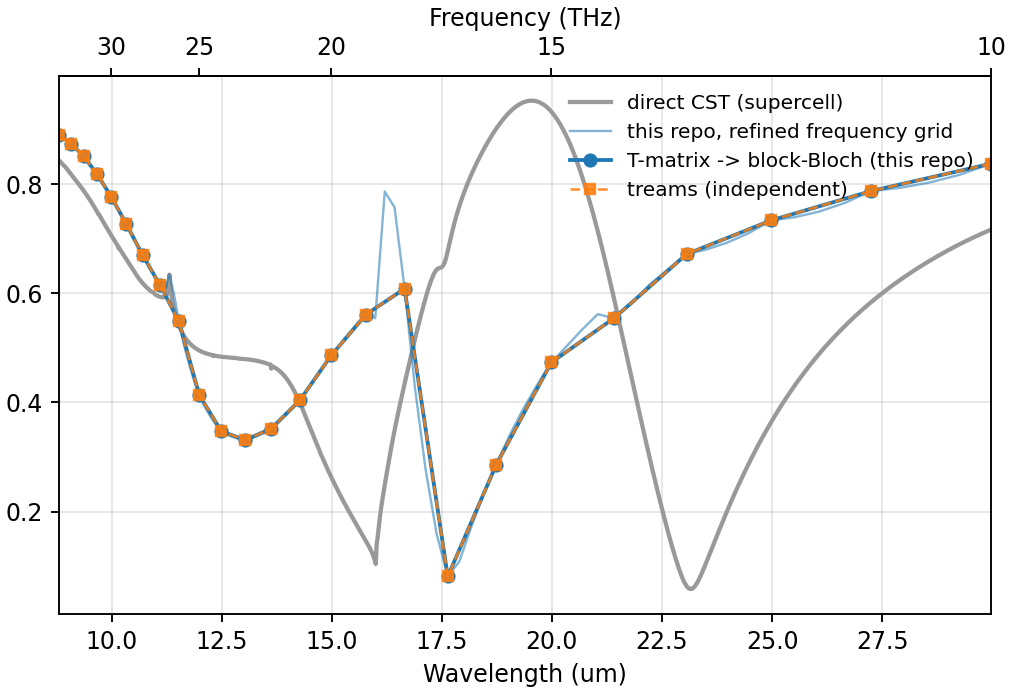
\includegraphics[width=\textwidth]{figs/s21_abcd_full.png}
      {\scriptsize\textit{\textcolor{gray}{a,b;c,d: this repo (blue) and treams (orange) are indistinguishable ---
      and both sit far from CST (grey).}}}\\[1ex]
      \colorbox{cardgold}{\parbox{0.95\textwidth}{\small\textit{\textbf{\textcolor{golddk}{Cross-code agreement validates
      the implementation. Only full-wave validates the physics.}}}}}
    \end{column}
  \end{columns}
\end{frame}

% ================================================================ 11 the cause
\begin{frame}{The cause: truncated addition theorem --- error contracts by only $\rho$ per order}
  \kicker{DIAGNOSIS  $\cdot$  THE MECHANISM}
  \begin{columns}[t]
    \begin{column}{0.50\textwidth}
      \begin{itemize}\small
        \item A T-matrix describes its atom only \emph{outside} the circumscribing sphere (radius $a$).
        \item Re-expanding neighbour $j$'s scattered field about atom $i$ converges like a geometric series in
              $\rho = (a_i + a_j)/d$: truncation at $l_{\max}$ leaves an error $\sim \rho^{\,l_{\max}}$.
      \end{itemize}
      \begin{center}\footnotesize
      \begin{tabular}{@{}clc@{}}
        \toprule
        $\rho$ & case & $l_{\max}$ needed for ${\sim}1\,\%$ \\
        \midrule
        0.652 & a,c;c,a & 11 \\
        0.809 & a,b;b,a & 22 \\
        \textcolor{bad}{\textbf{0.944}} & \textcolor{bad}{\textbf{a,b;c,d (B--D pair)}} & \textcolor{bad}{\textbf{80}} \\
        \textcolor{bad}{\textbf{0.989}} & \textcolor{bad}{\textbf{D alone (D--D pair)}} & \textcolor{bad}{\textbf{416}} \\
        \bottomrule
      \end{tabular}\\
      {\scriptsize\textit{\textcolor{gray}{Used: $l_{\max}=3$.}}}
      \end{center}
      \colorbox{cardgold}{\parbox{0.95\textwidth}{\footnotesize\textbf{\textcolor{golddk}{Silent by construction:}}
      the validity condition $a_i + a_j < d$ is \emph{satisfied} in every case (D--D: 7.912 vs 8.000\um).
      Marginally satisfied is worse than violated --- nothing warns.}}
    \end{column}
    \begin{column}{0.46\textwidth}
      \begin{center}
        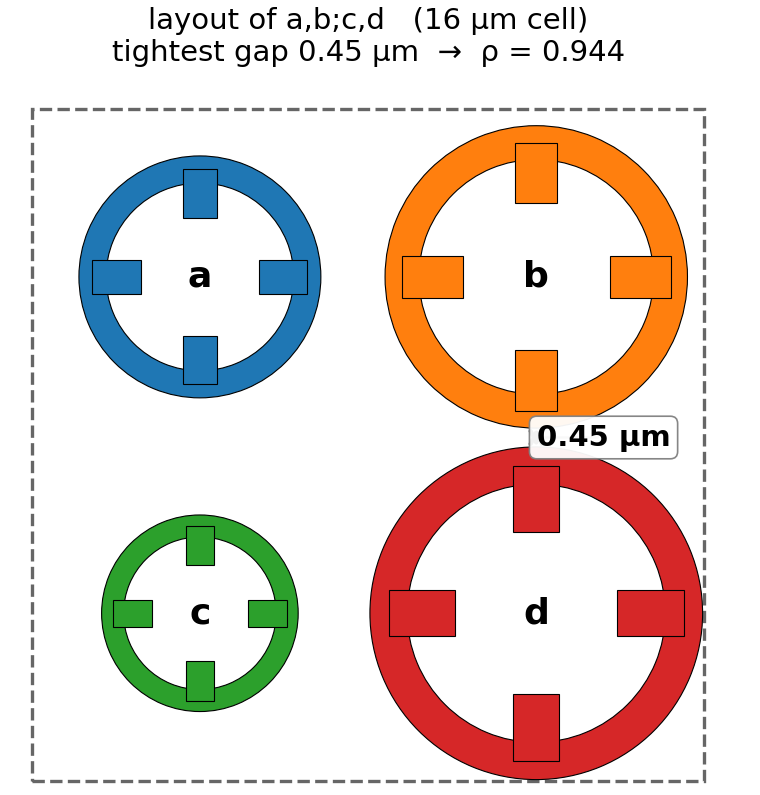
\includegraphics[width=0.48\textwidth]{figs/layout_abcd.png}\hfill
        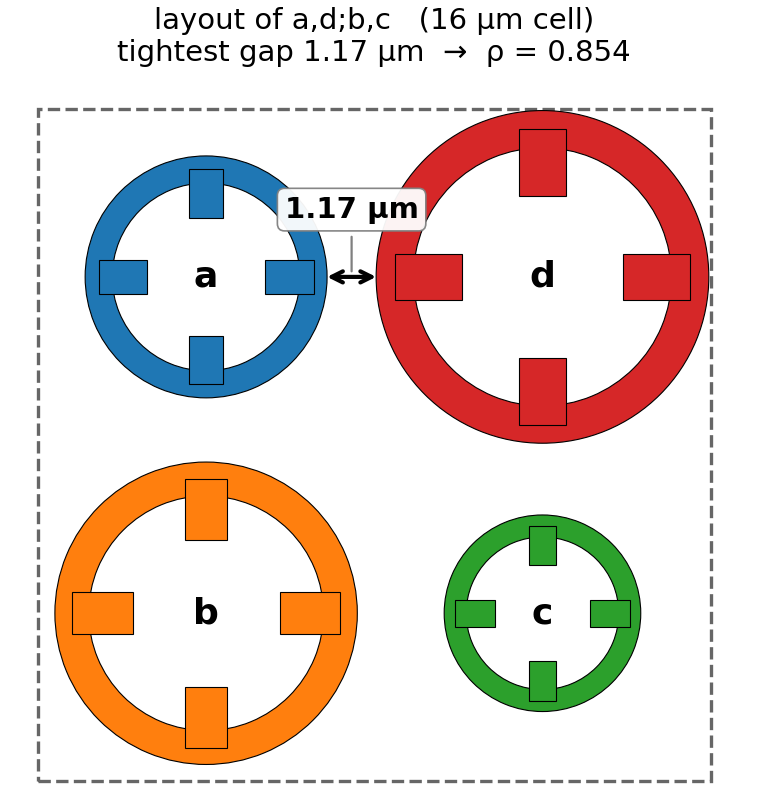
\includegraphics[width=0.48\textwidth]{figs/layout_adbc.png}
      \end{center}
      {\scriptsize\textit{\textcolor{gray}{The knob that matters: a,b;c,d puts B and D adjacent
      (gap 0.45\um, $\rho = 0.944$); a,d;b,c re-pairs the same four atoms (tightest gap 1.17\um,
      $\rho = 0.854$) and is $14\times$ more accurate.}}}
    \end{column}
  \end{columns}
\end{frame}

% ================================================================ 12 lmax dilemma
\begin{frame}{Raising $l_{\max}$ makes it worse: two errors move in opposite directions}
  \kicker{DIAGNOSIS  $\cdot$  THE DILEMMA}
  \begin{columns}[t]
    \begin{column}{0.48\textwidth}
      {\textcolor{good}{\textbf{$\downarrow$ truncation error}}}
      \begin{itemize}\small
        \item Falls like $\rho^{\,l_{\max}}$ --- at $\rho = 0.944$ each extra order buys a factor 0.944: $l_{\max}\approx 80$ for 1\,\%.
        \item At $l_{\max} = 3$--$5$ the neglected remainder of the B--D coupling is of order 1.
      \end{itemize}
    \end{column}
    \begin{column}{0.48\textwidth}
      {\textcolor{bad}{\textbf{$\uparrow$ noise amplification}}}
      \begin{itemize}\small
        \item The $l = 4,5$ rows of the measured $T$ sit at the extraction noise floor.
        \item The near-field lattice sum amplifies exactly those rows:
              $h_l(kp) \sim (2l-1)!!\,/\,(kp)^{\,l+1}$ --- $|W|$ at $l=3$ reaches 1025 at $\lambda \approx 30\um$
              vs 1.7 at 8.8\um: $227\times$ the dipole coupling there.
      \end{itemize}
    \end{column}
  \end{columns}
  \vspace{2ex}
  \colorbox{cardgold}{\parbox{0.96\textwidth}{\small\textbf{\textcolor{golddk}{Both measured, not predicted:}}
  \begin{itemize}\small
    \item Atom D's reconstruction is \emph{worse} at $l_{\max}=5$ than at $l_{\max}=3$ --- the noise term already dominates before truncation is fixed.
    \item The obvious internal check fails too: the $l_{\max}$ 3$\to$4$\to$5 spread is \emph{largest} for the most accurate cell (a,d;b,c), because the spread measures noise amplification, not geometry. There is no usable convergence warning.
  \end{itemize}}}
\end{frame}

% ================================================================ 13 the limitation
\begin{frame}{The limit is representational, not algorithmic}
  \kicker{THE LIMITATION}
  \begin{columns}[c]
    \begin{column}{0.42\textwidth}
      \begin{center}
      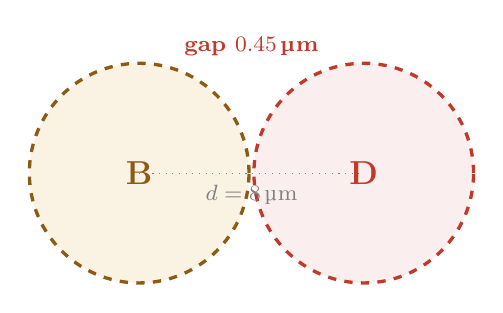
\begin{tikzpicture}[scale=0.62]
        \draw[dashed, very thick, golddk, fill=cardgold] (0,0) circle (2.25);
        \draw[dashed, very thick, bad, fill=bad!8] (4.6,0) circle (2.25);
        \draw[dotted, gray] (0,0) -- (4.6,0);
        \node[golddk, font=\bfseries\large] at (0,0) {B};
        \node[bad, font=\bfseries\large] at (4.6,0) {D};
        \node[gray, font=\footnotesize] at (2.3,-0.45) {$d = 8\um$};
        \node[bad, font=\footnotesize\bfseries] at (2.3,2.6) {gap $0.45\um$};
      \end{tikzpicture}\\[1ex]
      {\scriptsize\textit{\textcolor{gray}{Each T-matrix is valid only outside its dashed sphere ---
      the gap region belongs to neither expansion.}}}
      \end{center}
    \end{column}
    \begin{column}{0.54\textwidth}
      \begin{itemize}\small
        \item \textbf{A single-centre, $l_{\max}=3$ T-matrix has 30 modes. The field in a 0.45\um{} gap varies on the scale of the gap --- that information does not exist in those 30 numbers.}
        \item $\rho$ is fixed by geometry: circumscribing radii and centre distance. No solver setting, no lattice-sum method, no basis convention changes it.
        \item The hybridized gap mode (the measured red-shift) is reachable by the formalism only at $l_{\max}\approx 80$--$400$ --- far beyond what measured T-matrices support.
      \end{itemize}
    \end{column}
  \end{columns}
\end{frame}

% ================================================================ 14 why not aggregation
\begin{frame}{No modification of the aggregation alone can supply the missing physics}
  \kicker{WHY THE FIX IS NOT IN THE AGGREGATION}
  \textcolor{navy}{\textbf{Proof in one line --- the Neumann sandwich}}
  \begin{equation*}
    f \;=\; T a \;+\; T C T a \;+\; T C T C T a \;+\; \cdots
  \end{equation*}
  {\small Every lattice operator $C$ is sandwiched between two copies of the stored $T$.
  $T$ is zero outside $l \le 3$, so any higher-order content added to $C$ is annihilated on contact ---
  computing $C$ exactly, at any $l_{\max}$, changes nothing.}
  \vspace{1ex}
  \begin{columns}[t]
    \begin{column}{0.52\textwidth}
      \textcolor{navy}{\textbf{The other obvious fix dies on geometry}}\\
      {\footnotesize Merging the near-touching pair into one extracted super-atom makes a sphere that swallows the next neighbour:}\\[0.5ex]
      \begin{center}\footnotesize
      \begin{tabular}{@{}ccc@{}}
        \toprule
        merge & merged radius & worst $\rho$ vs rest \\
        \midrule
        B$+$D & 7.956\um & \textcolor{bad}{1.211 --- invalid} \\
        A$+$B & 7.596\um & \textcolor{bad}{1.292 --- invalid} \\
        C$+$D & 7.956\um & \textcolor{bad}{1.292 --- invalid} \\
        \bottomrule
      \end{tabular}\\
      {\scriptsize\textit{\textcolor{gray}{$\rho \ge 1$ violates the validity condition outright --- merging only works in sparse cells.}}}
      \end{center}
    \end{column}
    \begin{column}{0.44\textwidth}
      \colorbox{cardgold}{\parbox{0.95\textwidth}{\small\textbf{\textcolor{golddk}{Therefore}}\\[0.5ex]
      The missing gap-scale information must enter \emph{upstream} of the solve:
      the representation of each atom --- i.e.\ the extraction --- has to change,
      not the aggregation that consumes it.}}
    \end{column}
  \end{columns}
\end{frame}

% ================================================================ 15 the fix
\begin{frame}{The path forward: multi-centre representation --- make $\rho$ an algorithmic choice again}
  \kicker{THE PATH FORWARD}
  \begin{columns}[t]
    \begin{column}{0.52\textwidth}
      \begin{itemize}\small
        \item Replace one 4\um{} expansion centre by ${\sim}30$ sub-centres of radius $r_s \approx 0.5\um$ tiling the ring.
              Since $k\,r_s \approx 0.24$, each needs only dipoles ($l_{\max}=1$): ${\sim}180$ modes per atom, still a trivial dense solve.
        \item The pair convergence ratio becomes
              $\displaystyle \rho_{\text{sub}} = \frac{2 r_s}{g + 2 r_s}$
              --- set by a chosen radius, no longer by the fixed geometry.
      \end{itemize}
      \begin{center}\footnotesize
      \begin{tabular}{@{}cccl@{}}
        \toprule
        pair & gap $g$ & $\rho$ today & $\rho_{\text{sub}}$ at $r_s = 0.5\um$ \\
        \midrule
        B--D & 0.448\um & \textbf{0.944} & \textcolor{good}{\textbf{0.691}} \\
        A--D & 1.167\um & 0.854 & \textcolor{good}{0.461} \\
        D--D & 0.088\um & 0.989 & \textcolor{warn}{0.919 (graded radii near the gap)} \\
        \bottomrule
      \end{tabular}\\
      {\scriptsize\textit{\textcolor{gray}{B--D at $\rho_{\text{sub}} = 0.691$ would sit among the
      best-performing cells of the study ($\rho \approx 0.65$--$0.75$).}}}
      \end{center}
    \end{column}
    \begin{column}{0.44\textwidth}
      {\textcolor{good}{\textbf{${\sim}80\,\%$ already built}}}
      \begin{itemize}\footnotesize
        \item Block lattice sums take arbitrary per-cell positions (treams shift list)
        \item Multi-centre cluster operators exist (\texttt{cluster\_T})
        \item Change needed: dense per-atom blocks instead of diagonal $T$'s --- a data-model edit
      \end{itemize}
      \vspace{1ex}
      {\textcolor{bad}{\textbf{The real cost: extraction}}}
      \begin{itemize}\footnotesize
        \item $\ge 180$ independent excitations per atom
        \item Plane waves are too smooth --- near-field (dipole) sources must join the illumination set
        \item A new CST protocol; the existing conditioning machinery is the right design tool
      \end{itemize}
    \end{column}
  \end{columns}
\end{frame}

% ================================================================ 16 closing
{\setbeamercolor{background canvas}{bg=navy}
\begin{frame}[plain]
  \vspace{0.8cm}
  {\footnotesize\bfseries\textcolor{white!70!navy}{GUARDRAILS NOW  $\cdot$  TAKEAWAYS}}\\[1ex]
  {\Large\bfseries\textcolor{white}{What to do while the representation is rebuilt}}\\[3ex]
  \begin{columns}[t]
    \begin{column}{0.32\textwidth}
      {\textcolor{gold}{\textbf{Gate on $\rho$}}}\\[0.5ex]
      {\footnotesize\textcolor{white!85!navy}{Warn above 0.85, refuse above 0.95 (with \texttt{-{}-force}).
      The $\eta$-split already refuses rather than guesses --- extend the policy.
      Blocked only on storing the circumscribing radius in \texttt{tmat.h5}.}}
    \end{column}
    \begin{column}{0.32\textwidth}
      {\textcolor{gold}{\textbf{Design around it}}}\\[0.5ex]
      {\footnotesize\textcolor{white!85!navy}{Never place the two largest atoms adjacent:
      a,d;b,c vs a,b;c,d is $14\times$ better for free --- same atoms, same lattice.}}
    \end{column}
    \begin{column}{0.32\textwidth}
      {\textcolor{gold}{\textbf{Denoise, then $l_{\max}$}}}\\[0.5ex]
      {\footnotesize\textcolor{white!85!navy}{Symmetry-average the noisy $l = 4,5$ rows before any
      $l_{\max}$ raise. Helps the $\rho \approx 0.85$ band; cannot reach 0.944.}}
    \end{column}
  \end{columns}
  \vspace{3ex}
  {\color{white!30!navy}\rule{\textwidth}{0.5pt}}\\[1.5ex]
  {\small\textcolor{white}{%
  \textcolor{gold}{\textbf{1}}\; Validated: composing metasurfaces from measured atoms is essentially free below $\rho \approx 0.85$ --- accuracy is set by the inputs, not the method.\\[0.8ex]
  \textcolor{gold}{\textbf{2}}\; The failures (a,b;c,d, a,c;d,b, atom D) are one diagnosed mechanism --- slow convergence of the truncated addition theorem across sub-\textmu m gaps --- not noise, and not a bug: treams reproduces them to $10^{-15}$.\\[0.8ex]
  \textcolor{gold}{\textbf{3}}\; The fix is representational, not algorithmic: the aggregation provably cannot supply the missing gap physics; a multi-centre extraction can.}}
\end{frame}}

\end{document}
